\documentclass[a4paper, 12pt]{article}

\usepackage[table,xcdraw]{xcolor}
\usepackage[left=2.5cm, right=1.5cm, top=1.5cm, bottom=1.5cm]{geometry}
\usepackage{graphicx}
\usepackage{xcolor}
\usepackage{mdframed}
\usepackage { amsmath , amssymb , amsthm }
\usepackage[T2A]{fontenc}
\usepackage[utf8]{inputenc}
\usepackage[english,russian]{babel}
\usepackage{listings}
\usepackage{setspace}
\usepackage{amsmath}
\usepackage{float}
\usepackage{multirow}
\usepackage{lscape}


\onehalfspacing
\renewcommand{\familydefault}{\sfdefault}
% \renewcommand{\familydefault}{\sffamily}

\graphicspath{{img/}}
\DeclareGraphicsExtensions{.pdf,.png,.jpg}


\begin{document}
\begin{titlepage}
  \begin{center}
    \MakeUppercase{Министерство науки и высшего образования Российской Федерации} \\
    \MakeUppercase{ФГБОУ ВО Алтайский госудаственный университет}
    \vspace{0.25cm}
    
	  Институт цифровых технологий, электроники и физики
    
    Кафедра вычислительной техники и электроники
    \vfill
    
    {\LARGE Лабораторная работа №6. Задача о рационе}\\[5mm]
    \textsc{(Отчёт по лабораторным работам по курсу <<Методы оптимизации>>. \\13 вариант)}
  \bigskip

\end{center}
\vfill

\newlength{\ML}
\settowidth{\ML}{«\underline{\hspace{0.7cm}}» \underline{\hspace{1cm}}}
\hfill
\begin{minipage}{0.45\textwidth}
  Выполнил: ст. 595 гр.:\\
  \underline{\hspace{\ML}} Д.\,В.~Осипенко\\
  Проверил: к.ф-м. наук, доцент каф. ВТиЭ\\
  \underline{\hspace{\ML}} В.\,И.~Иордан\\
  «\underline{\hspace{0.7cm}}» \underline{\hspace{2cm}} \the\year~г.
\end{minipage}%
\vfill

\begin{center}
  Барнаул, \the\year~г.
\end{center}
\end{titlepage}

\newpage
\section{Краткие теоретические сведения}
Задача линейного программироваия состоит в находжении $\vec{x}$, который минимизирует целевую функцию $f^Tx$, где $f$ - вектор коэффициентов, и удовлетворяет заданным линейным ограничениям: неравенствам $Ax\leq b$ и равенствам $A_{eq}x = b_{eq}$. Кроме того, могут быть поставленны двусторонние покомпонентные ограничения в векторной форме: $lb\leq x \leq ub$.

В задачах оптимизации могут быть заданы не все типы ограничений, например, ограничения-равенства могут отсутствовать.
\section{Решение индивидуального задания. 13 вариант.}
Изветсны минимальные суточные потребности человека, в зависимости от пола и возраста, в питальных веществах и незаменимых компонентах. В табл.3 прведены содержание питательных веществ и незаменимых компонентов в 100 г. продукта. Стоимость 100 г. продуктов, включенных в диету, и предельные количества по каждому сформировать самостоятельно. Требуется рассчитать суточную диету, чтобы, с одной стороны, обеспечить минимально необходимое количество питательных веществ и незаменимых компонентов, а с другой - минимизировать стоимость разработанной диеты. При этом необходимо посчитать энергетическую ценность полученной диеты. \\

Список продуктов (13 вариант):
\textit{Крупа кукурузная, Хлеб ржаной из сеяной муки, Пряники заварные, Сыр костромской, Куры, Треска, Масло сливочное, Грейпфрут, Свекла, Яблоки.}\\

\begin{center}
  Табл 6.1 Данные к задаче
\end{center}
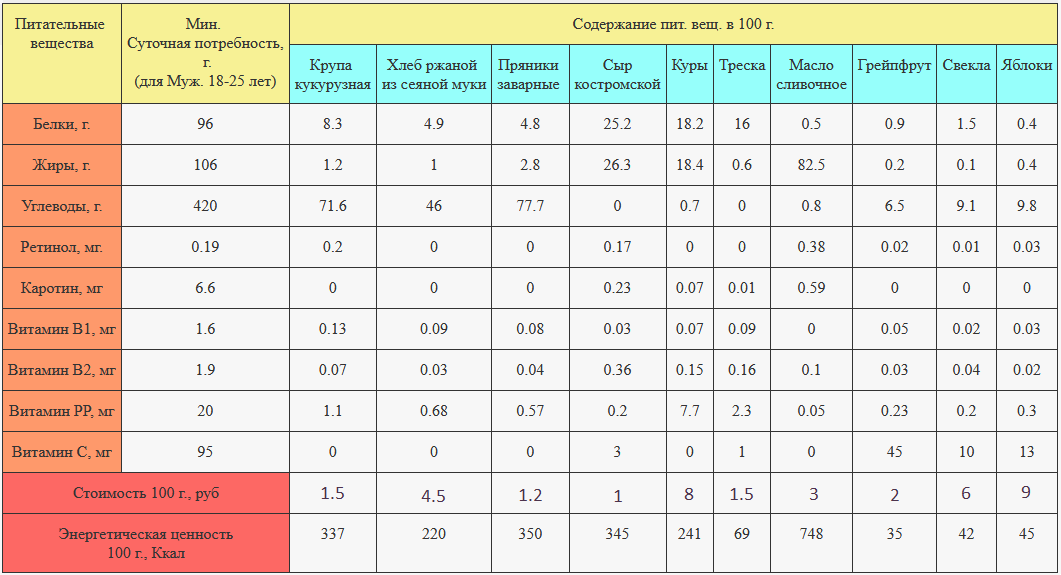
\includegraphics[width=\textwidth]{6-5.png}\\

Решим классическую задачу линейного программирования о составлении рациона питания.

Пусть имеется 10 видов продуктов, содержащих 9 питательных веществ и незаменимых компанентов. Кроме того, известны: ежесуточная минимальная потребность организма в веществах, стоимость и энергетическая ценность (Ккал) 100 г. продукта. Требуется расчитать суточную диету так, чтобы обеспечить необходимо количество питательных веществ и незаменимых компонетов при минимальных затратах на продукты. Найти калорийность.

Требуется минимизировать затраты на приобретение продуктов. Очевидно, что количество приобретаемых продуктов не может быть отрицательным.

\begin{align*}
  Z(X) = \frac{1}{100}\sum_{j=0}^{10} c_jx_j \rightarrow \min
\end{align*}\\

Поскольку линейные ограничения содержат "меньше или равно", а количество ингредиентов в рационе недолжно быть менее заданных величин, то следует изменить знаки обеиз частей системы\\
\begin{align*}
  A=\begin{vmatrix}
    -8.3 & -4.9 & -4.8 & -25.2 & -18.2 & -16 & -0.5 & -0.9 & -1.5 & -0.4 \\
    -1.2 & -1 & -2.8 & -26.3 & -18.4 & -0.6 & -82.5 & -0.2 & -0.1 & -0.4 \\
    -71.6 & -46 & -77.7 & 0 & -0.7 & 0 & -0.8 & -6.5 & -9.1 & -9.8 \\
    -0.2 &  0 & 0 & -0.17 & 0 & 0 & -0.38 & -0.02 & -0.01 & -0.03 \\
    0 & 0 & 0 &-0.23 & -0.07 & -0.01 & -0.59 & 0 & 0 & 0 \\
    -0.13 & -0.09 & -0.08 & -0.03& -0.07 & -0.09 & 0 & -0.05 & -0.02 & -0.03 \\
    -0.07 & -0.03 & -0.04 & -0.36 & -0.15 & -0.16 & -0.1 & -0.03 & -0.04 & -0.02 \\
    -1.1 & -0.68 & -0.57 & -0.2 & -7.7 & -2.3 & -0.05 & -0.23 & -0.2 & -0.3 \\
    0 & 0 & 0 & -3 & 0 & -1 & 0 & -45 & -10 & -13 
\end{vmatrix}
\end{align*}
\begin{align*}
  b=\begin{vmatrix}
    -9600 \\ -10600 \\ -42000 \\ -19 \\ -660 \\ -160 \\ -190 \\ -2000 \\ -9500
  \end{vmatrix}
\end{align*}

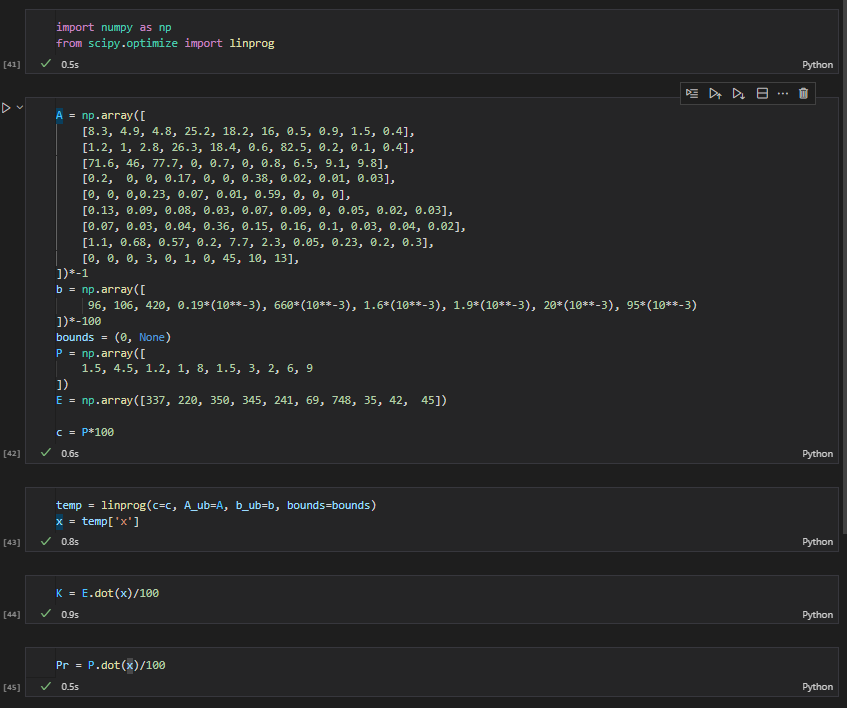
\includegraphics[width=\textwidth]{6-6.png}
\begin{center}
  Программа на Python3
\end{center}
\begin{align*}
  K = 3010.7888(\textit{Ккал}), \quad Pr = 9.9093(\textit{руб})
\end{align*}

\end{document}
